% complex lecture
\documentclass{report}

\usepackage{fancyhdr}
\usepackage{amsmath,amsfonts,amsthm,amssymb,mathtools}
\usepackage{geometry}
\usepackage{etoolbox}
\usepackage{xifthen}
\usepackage{mathrsfs, graphics}
\usepackage{tikz}
\usepackage{tikzsymbols}
\usepackage{marginnote, xcolor}
\usepackage{graphicx}
\usepackage{footnote}
\usetikzlibrary{patterns, patterns.meta}
% \usepackage{fourier-orns}
% \usepackage{fontawesome5}
\usepackage{tcolorbox}
\tcbuselibrary{skins}
\tcbuselibrary{breakable}

% Geometry

\geometry{a4paper, left=2cm, right=4cm}
\linespread{1.5}

% colors 

\definecolor{denisBicep}{RGB}{216, 168, 146} 
\definecolor{larratBicep}{RGB}{208, 153, 117} 
\definecolor{graylol}{RGB}{144, 132, 124} 


% \definecolor{denisBicep}{RGB}{26, 48, 146} 
% \definecolor{larratBicep}{RGB}{98, 43, 117} 
% \definecolor{graylol}{RGB}{44, 2, 14} 

% \definecolor{denisBicep}{RGB}{60, 48, 160} 
% \definecolor{larratBicep}{RGB}{0, 03, 70} 
% \definecolor{graylol}{RGB}{40, 200, 4} 

% fancy hdr

\pagestyle{fancy}                             

\newcommand{\lecture}[3]
{      
  
  \ifthenelse{\isempty{#3}}{
    \def\@lecture{Lecture #1\tt\hfill#2}
    \def\ps{Lecture #1}
  }{
    \def\@lecture{Lecture #1: #3\tt\hfill#2}
    \def\ps{Lecture #1: #3}
  } 
  \subsection*{\@lecture}
}

\fancyhead[R]{\ps}
\fancyfoot[L]{\leftmark}
\fancyfoot[C]{}
\fancyfoot[R]{\thepage}

% general background

\newcommand{\divider}
{
	\begin{center}
	\begin{tikzpicture}
		\draw[black, dashed] (0.25*\textwidth, 0) -- (0.75*\textwidth, 0);
		\node[rotate = 360 - 90, xshift = -0.6pt, yshift = 1pt] at (0.25*\textwidth,0) { };
		\node[rotate = 90, xshift = -0.6pt, yshift = 1pt] at (0.75*\textwidth,0) { };
	\end{tikzpicture}
	\end{center}
}

% new if definitions for chapter :c

\newif\ifchapterpage
\chapterpagefalse

% hook \chapter and then we set the flag :>

\let\oldchapter\chapter
\renewcommand{\chapter}{%
  \global\chapterpagetrue
  \oldchapter
}

\AddToHook{shipout/background}{
  \begin{tikzpicture}[remember picture, overlay]

    \ifchapterpage
    \draw[draw=black,fill=larratBicep!35, opacity=0.5] ([yshift = -(\paperheight - \textheight)/2 + 1.5cm, 
                                         xshift = (\paperwidth - \textwidth)/2 - 1.5cm]current page.north west) rectangle
                                          ([yshift = (\paperheight - \textheight)/2 + 0.5cm ,
                                          xshift = -(\paperwidth - \textwidth)/2 - 0.5cm]current page.south east);
    \draw[draw=larratBicep!50, step=5mm, opacity=0.5] ([yshift = -(\paperheight - \textheight)/2 + 1.5cm, 
                                          xshift = (\paperwidth - \textwidth)/2 - 1.5cm]current page.north west) grid
                                          ([yshift = (\paperheight - \textheight)/2 + 0.5cm ,
                                          xshift = -(\paperwidth - \textwidth)/2 - 0.5cm]current page.south east);
    \draw[draw=black] ([yshift = -(\paperheight - \textheight)/2 + 1.5cm, 
                                         xshift = (\paperwidth - \textwidth)/2 - 1.5cm]current page.north west) rectangle
                                         ([yshift = (\paperheight - \textheight)/2 + 0.5cm ,
                                         xshift = -(\paperwidth - \textwidth)/2 - 0.5cm]current page.south east);
      \global\chapterpagefalse

    \else         

    \draw[draw=black,fill=larratBicep!35, opacity=0.5] ([yshift = -(\paperheight - \textheight)/2 + 1.5cm, 
                                         xshift = (\paperwidth - \textwidth)/2 - 1.5cm]current page.north west) rectangle
                                          ([yshift = (\paperheight - \textheight)/2 + 0.5cm ,
                                          xshift = -(\paperwidth - \textwidth)/2 - 0.5cm]current page.south east);
    \draw[draw=larratBicep!50, step=5mm, opacity=0.5] ([yshift = -(\paperheight - \textheight)/2 + 1.5cm, 
                                          xshift = (\paperwidth - \textwidth)/2 - 1.5cm]current page.north west) grid
                                          ([yshift = (\paperheight - \textheight)/2 + 0.5cm ,
                                          xshift = -(\paperwidth - \textwidth)/2 - 0.5cm]current page.south east);
    \draw[draw=black, opacity=0.5] ([yshift = -(\paperheight - \textheight)/2 + 1.5cm, 
                                         xshift = (\paperwidth - \textwidth)/2 - 1.5cm]current page.north west) rectangle
                                         ([yshift = (\paperheight - \textheight)/2 + 0.5cm ,
                                         xshift = -(\paperwidth - \textwidth)/2 - 0.5cm]current page.south east);
    \fi

  \end{tikzpicture}
}

% parenthesis check

\newcommand{\maybep}[1]{ 
  \if\relax\detokenize{#1}\relax
  \else
    \ (#1)
  \fi
}

% tcolorbox environments

\usetikzlibrary{patterns}

\newtcolorbox[auto counter, number within=section]{theorem}[1][]           
{title=Theorem \thetcbcounter\maybep{#1}: ,drop lifted shadow=black,enhanced,colframe=blue!50!black,colback=blue!25!denisBicep!50,attach title to upper = {\ },
coltitle=blue!50!black,fonttitle=\upshape\bfseries,fontupper=\itshape,
sharp corners = all,boxrule = 0pt,
breakable,
underlay = {\draw[step=5mm,
  draw = blue!25!denisBicep!60] (interior.north east)
grid (interior.south west);
\draw[blue!25!denisBicep!60] ([xshift = 0.45cm]interior.north west) -- ([yshift = -0.28cm, xshift = 0.48cm]interior.north west); %  -----
\draw[blue!25!denisBicep!60] ([yshift = -0.35cm]interior.north west) -- ([yshift = -0.28cm, xshift = 0.48cm]interior.north west); % -
\path[fill = blue!40!denisBicep!40,drop shadow={opacity = 0.55, shadow xshift = .0ex, shadow yshift = -.4ex, shadow scale = 1, 
 }]
([xshift = 0.45cm]interior.north west) -- ([yshift = -0.28cm, xshift = 0.48cm]interior.north west) -- 
   ([yshift = -0.35cm]interior.north west) -- ([xshift = 0.45cm]interior.north west) ;
                                                                                                                              % -  x
\fill[fill=larratBicep!35!white!50] ([yshift = -0.35cm]interior.north west) -- ([xshift = 0.45cm]interior.north west) -- (interior.north west);

\draw[larratBicep!35] ([yshift = -0.35cm]interior.north west) -- (interior.north west);
\draw[larratBicep!35!white!50] ([yshift = -0.35cm]interior.north west) -- ([xshift = 0.45cm]interior.north west);
\draw[larratBicep!35!white!50] ([xshift = 0.45cm]interior.north west) -- (interior.north west);
}
}

\newtcolorbox[use counter from=theorem]{proposition}[1][]           
{title=Proposition \thetcbcounter\maybep{#1}: ,drop lifted shadow=black,enhanced,colframe=denisBicep!35,colback=denisBicep!35,attach title to upper = {\ },
breakable,
underlay = { 
  \draw[larratBicep!60] ([xshift = 0.45cm]interior.north west) -- ([yshift = -0.28cm, xshift = 0.48cm]interior.north west); %  -----
  \draw[larratBicep!60] ([yshift = -0.35cm]interior.north west) -- ([yshift = -0.28cm, xshift = 0.48cm]interior.north west); % -
  \path[fill = larratBicep!45,drop shadow={opacity = 0.55, shadow xshift = .0ex, shadow yshift = -.4ex, shadow scale = 1, 
   }]
  ([xshift = 0.45cm]interior.north west) -- ([yshift = -0.28cm, xshift = 0.48cm]interior.north west) -- 
     ([yshift = -0.35cm]interior.north west) -- ([xshift = 0.45cm]interior.north west) ;
                                                                                                                                % -  x
  \fill[fill=larratBicep!35!white!50] ([yshift = -0.35cm]interior.north west) -- ([xshift = 0.45cm]interior.north west) -- (interior.north west);

  \draw[larratBicep!35] ([yshift = -0.35cm]interior.north west) -- (interior.north west);
  \draw[larratBicep!35!white!50] ([yshift = -0.35cm]interior.north west) -- ([xshift = 0.45cm]interior.north west);
  \draw[larratBicep!35!white!50] ([xshift = 0.45cm]interior.north west) -- (interior.north west);
},
coltitle=red!50!black,fonttitle=\upshape\bfseries,fontupper=\itshape,
sharp corners = all,boxrule = 0pt,
underlay = {\draw[step=5mm,
  draw = larratBicep!45] (interior.north east)
grid (interior.south west);}
}

\newtcolorbox[auto counter, number within=section]{definition}[1][]           
{title=Definition \thetcbcounter\maybep{#1}: ,drop lifted shadow=black,enhanced,colframe=red!25,colback=red!25!larratBicep!50,attach title to upper = {\ },
breakable,
coltitle=red!50!black,fonttitle=\upshape\bfseries,fontupper=\itshape,
sharp corners = all,boxrule = 0pt,
underlay = {\draw[step=5mm,
  draw = red!25!larratBicep!60] (interior.north east)
grid (interior.south west);
  \draw[red!35] ([xshift = 0.45cm]interior.north west) -- ([yshift = -0.28cm, xshift = 0.48cm]interior.north west); %  -----
  \draw[red!35] ([yshift = -0.35cm]interior.north west) -- ([yshift = -0.28cm, xshift = 0.48cm]interior.north west); % -
  \path[fill = red!35,drop shadow={opacity = 0.55, shadow xshift = .0ex, shadow yshift = -.4ex, shadow scale = 1, 
   }]
  ([xshift = 0.45cm]interior.north west) -- ([yshift = -0.28cm, xshift = 0.48cm]interior.north west) -- 
     ([yshift = -0.35cm]interior.north west) -- ([xshift = 0.45cm]interior.north west) ;
                                                                                                                                % -  x
  \fill[fill=larratBicep!35!white!50] ([yshift = -0.35cm]interior.north west) -- ([xshift = 0.45cm]interior.north west) -- (interior.north west);

  \draw[larratBicep!30] ([yshift = -0.35cm]interior.north west) -- (interior.north west);
  \draw[larratBicep!35!white!50] ([yshift = -0.35cm]interior.north west) -- ([xshift = 0.45cm]interior.north west);
  \draw[larratBicep!35!white!50] ([xshift = 0.45cm]interior.north west) -- (interior.north west);
}
}

\newtcolorbox[auto counter, number within=section]{remark}
{title=Remark \ding{46} \\\noindent,drop lifted shadow=black,enhanced,colframe=yellow!25,colback=yellow!25!larratBicep!50,attach title to upper = {\ },
breakable,
coltitle=yellow!50!black,fonttitle=\upshape\bfseries,fontupper=\normalfont,
sharp corners = all,boxrule = 0pt,
underlay = {\draw[step=5mm,
  draw = yellow!25!larratBicep!60] (interior.north east)
grid (interior.south west);
  \draw[larratBicep!35] ([xshift = 0.45cm]interior.north west) -- ([yshift = -0.28cm, xshift = 0.48cm]interior.north west); %  -----
  \draw[larratBicep!35] ([yshift = -0.35cm]interior.north west) -- ([yshift = -0.28cm, xshift = 0.48cm]interior.north west); % -
  \path[fill = yellow!50!larratBicep!50,drop shadow={opacity = 0.55, shadow xshift = .0ex, shadow yshift = -.4ex, shadow scale = 1, 
   }]
  ([xshift = 0.45cm]interior.north west) -- ([yshift = -0.28cm, xshift = 0.48cm]interior.north west) -- 
     ([yshift = -0.35cm]interior.north west) -- ([xshift = 0.45cm]interior.north west) ;
                                                                                                                                % -  x
  \fill[fill=larratBicep!35!white!50] ([yshift = -0.35cm]interior.north west) -- ([xshift = 0.45cm]interior.north west) -- (interior.north west);

  \draw[larratBicep!35] ([yshift = -0.35cm]interior.north west) -- (interior.north west);
  \draw[larratBicep!35!white!50] ([yshift = -0.35cm]interior.north west) -- ([xshift = 0.45cm]interior.north west);
  \draw[larratBicep!35!white!50] ([xshift = 0.45cm]interior.north west) -- (interior.north west);
}
}

\usetikzlibrary{shadows}
\newtcolorbox[use counter from=theorem]{corollary}[1][]           
{title=Corollary \thetcbcounter\maybep{#1}: ,drop lifted shadow=black,enhanced,colframe=green!35!black!15,colback=green!35!black!15!denisBicep!45,attach title to upper = {\ },
coltitle=green!25!black,fonttitle=\upshape\bfseries,fontupper=\itshape,
breakable,
sharp corners = all,boxrule = 0pt,
underlay = {\draw[step=5mm,
  draw = green!40!black!30!denisBicep!50] (interior.north east)
grid (interior.south west);

  \draw[green!40!black!35] ([xshift = 0.45cm]interior.north west) -- ([yshift = -0.28cm, xshift = 0.48cm]interior.north west); %  -----
  \draw[green!40!black!35] ([yshift = -0.35cm]interior.north west) -- ([yshift = -0.28cm, xshift = 0.48cm]interior.north west); % -
  \path[fill = green!35!black!20,drop shadow={opacity = 0.55, shadow xshift = .0ex, shadow yshift = -.4ex, shadow scale = 1, 
   }]
  ([xshift = 0.45cm]interior.north west) -- ([yshift = -0.28cm, xshift = 0.48cm]interior.north west) -- 
     ([yshift = -0.35cm]interior.north west) -- ([xshift = 0.45cm]interior.north west) ;
                                                                                                                                % -  x
  \fill[fill=larratBicep!35!white!50] ([yshift = -0.35cm]interior.north west) -- ([xshift = 0.45cm]interior.north west) -- (interior.north west);

  \draw[larratBicep!35] ([yshift = -0.35cm]interior.north west) -- (interior.north west);
  \draw[larratBicep!35!white!50] ([yshift = -0.35cm]interior.north west) -- ([xshift = 0.45cm]interior.north west);
  \draw[larratBicep!35!white!50] ([xshift = 0.45cm]interior.north west) -- (interior.north west);
}
}

\newtcolorbox[auto counter]{example}
{title=Example: ,drop fuzzy shadow=black,enhanced,colframe=gray!50!black,colback=gray!35,attach title to upper = {\ },
coltitle=gray!50!black,fonttitle=\upshape\bfseries,fontupper=\itshape,
breakable,
sharp corners = all,boxrule = 0pt,
underlay = {\draw[step=5mm,
  draw = gray!40!black!30] (interior.north east)
grid (interior.south west);}
}

% margi note configuration

\makeatletter

\setlength{\marginparsep}{18pt}
\renewcommand*{\marginfont}{\color{blue}}
\makeatother

% other (exercise enviroment)

\newcommand{\exercise}[1][]{
    \def\@exercise{#1}
    \subsection*{Exercise #1}
}

\newcommand{\subexercise}[1][]{
    \subsubsection*{Exercise \@exercise.#1}
}

% macros

\newcommand{\integral}[4]{\int\limits_{#1}^{#2} #4 d#3}
\newcommand{\limit}[3]{\lim\limits_{#1 \rightarrow #2} #3}
\newcommand{\strone}[2]{\left[ \begin{gathered}#1\\ #2\end{gathered} \right] }
\newcommand{\strtwo}[2]{\left\{ \begin{gathered}#1\\ #2\end{gathered} \right\} }
\newcommand{\strthree}[2]{\left\lfloor \begin{gathered}#1\\ #2\end{gathered} \right\rfloor }

\newcommand{\startbf}[1]{\text{\bfseries{#1}}}
\newcommand{\sett}[1]{\left\{ #1 \right\}}
\newcommand{\thesis}[1]{\left( #1 \right)}
\newcommand{\brkt}[1]{\left[ #1 \right]}
\newcommand{\floor}[1]{\left\lfloor #1 \right\rfloor}

\DeclareMathOperator{\img}{im} 
\DeclareMathOperator{\Img}{Im} 
\DeclareMathOperator{\coker}{coker} 
\DeclareMathOperator{\Coker}{Coker} 
\DeclareMathOperator{\Ker}{Ker} 
\DeclareMathOperator{\rank}{rank}
\DeclareMathOperator{\Spec}{Spec} 
\DeclareMathOperator{\Tr}{Tr} 
\DeclareMathOperator{\pr}{pr} 
\DeclareMathOperator{\ext}{ext} 
\DeclareMathOperator{\pred}{pred} 
\DeclareMathOperator{\dom}{dom} 
\DeclareMathOperator{\ran}{ran} 
\DeclareMathOperator{\Hom}{Hom} 
\DeclareMathOperator{\Mor}{Mor} 
\DeclareMathOperator{\End}{End} 

\newcommand{\lm}{\ensuremath{\lambda}}
\newcommand{\eps}{\ensuremath{\epsilon}}
\newcommand{\veps}{\ensuremath{\varepsilon}}
\newcommand{\al}{\ensuremath{\alpha}}
\newcommand{\bb}{\ensuremath{\beta}}
\newcommand{\cc}{\ensuremath{\gamma}}
\newcommand{\dd}{\ensuremath{\delta}}
\newcommand{\DD}{\ensuremath{\Delta}}
\newcommand{\ff}{\ensuremath{\phi}}
\newcommand{\FF}{\ensuremath{\varphi}}

\newcommand{\RR}{\mathbb{R}}
\newcommand{\RO}{\mathcal{R}}
\newcommand{\EE}{\mathbb{E}}
\newcommand{\CC}{\mathbb{C}}
\newcommand{\RW}{\mathbb{R}^2}
\newcommand{\RT}{\mathbb{R}^3}
\newcommand{\RN}{\mathbb{R}^n}
\newcommand{\DS}{\mathcal{D}}

\newcommand{\KK}{\mathbb{K}}
\newcommand{\KW}{\mathbb{K}^2}
\newcommand{\KT}{\mathbb{K}^3}
\newcommand{\KN}{\mathbb{K}^n}

\newcommand{\NN}{\mathbb{N}}

\newcommand{\PS}{\mathcal{P}}
\newcommand{\AS}{\mathcal{E}}
\newcommand{\FS}{\mathcal{F}}
\newcommand{\LS}{\mathcal{L}}
\newcommand{\MS}{\mathcal{M}}

\usepackage{mathpazo}
\usepackage{pifont}
\usepackage{fourier-orns}
\usepackage{hyperref}
\usepackage{ulem}

% \newtcolorbox{remark}{
%   colback=yellow!10,
%   colframe=yellow!60!black,
%   title=\textbf{Remark},
%   fonttitle=\sffamily,
%   boxrule=0.5pt,
%   arc=2mm
% }


\begin{document}

\begin{titlepage}
  \begin{center}
    \vspace*{2cm}
    {\LARGE Complex Analysis Lecture Notes}
    \\
    \vspace{1cm}
    {\large \it Hand written summary from lectures}
    \normalfont
  \end{center}
  \rule{\textwidth}{0.4pt}
  \begin{center}
    \textbf{Acknowledgment}
  \end{center}
  \begin{center}
    Special thanks to my professor \textsc{\textcolor{purple}{\large Mr.Bakir Farhi}}\normalfont,
    who gave the lectures and explanations,
    this work wouldn't exist without his teaching. here is the link to his website:
  \end{center}
    \begin{center}
  \href{
  http://farhi.bakir.free.fr/home/index-fr.html
  }{\texttt{ \large
  http://farhi.bakir.free.fr/home/index-fr.html}}
\end{center}
\vspace{0.4cm}
  \begin{center}
  \rule{\textwidth}{0.4pt}
    \textbf{Disclaimer}
  \end{center}
  \begin{center}
    These notes were written in real-time
    during the lectures,
    \underline{this is not the final version}, yet. so they may contain :
    \begin{itemize}
      \item
        Incomplete or incorrect information.
      \item
        Typos, transcription mistakes, or missing content.
      \item
        Interpretations or notations that reflect my own understanding.
        at the moment
    \end{itemize}
  \end{center}
  \vfill
  \begin{center}
    \it
    \large
    Please double check anything important with official
    material or trusted sources. \normalfont
  \end{center}
\end{titlepage}

\begin{titlepage}
  \begin{center}
    If you spot an error feel free to open an issue or
    submit a pull request, or contact me
    via gmail :
  \end{center}
  \begin{center}
    \normalfont
    \texttt{
      \large kara.abderahmane@nhsm.edu.dz
      \normalfont
    }
  \end{center}
  \noindent \textbf{Notes on Contribution : } \\
  This document is a collaborative effort.
  students who contribute by reporting errors or helping to complete the content
  will be credited in the next page as contributors in future versions,
  your help is appreciated and helps improve this document for everyone.
\end{titlepage}
\begin{titlepage}
  \newpage
  \normalfont
  \vfill
  \begin{center}
    \href{https://github.com/Kapa9102}{\textbf{My Github Page}}\\
    \vspace{0.8cm}
    Last Update : 2025-10-11
  \end{center}
  \begin{tcolorbox}[enhanced, colback=yellow!70!orange!20!white, sharp corners, boxrule=1pt,
    attach boxed title to top center = {yshift = -10pt, xshift = 0pt}, colbacktitle=yellow!30!orange!20!white,
    boxed title style = {boxrule=0pt, arc=4pt}, title=\sc\textcolor{black}{Contributors}]
    \begin{center}
      \it Main Writer \hfill \normalfont  \textsc{Kara Abderahmane}  \\
      \vspace{0.5cm}
      \tt Main Drawer \hfill \normalfont  \tt{Haddar Noureddine}  \\
    \end{center}
  \end{tcolorbox} 
  \vfill
  \begin{center}
   \textsc{\textcolor{purple}{\large ArmWrestling4Ever}}\normalfont
  \end{center}
\end{titlepage}
\tableofcontents
% lec1.tex 
\chapter{Power Series}
\lecture{1}{08:06 AM Mon, Sep 29 2025}{} 

\begin{definition}[Power Series]
  A power series is a formal series of the form 
  $\sum_{n=0}^{\infty} a_{n}z^{n} $, where $a_{n} \in  \CC $ for all
  $n \in \NN_0$. \\
  More generally, given $z_0 \in \CC  $, a power series 
  centered at  $z_0 $ is a formal series of the form: 
  \[
  \sum_{n=0}^{\infty} a_{n}(z-z_0) ^{n},
  \]
  where $a_{n} \in \CC  \quad (\forall n \in \NN_0)  $ 
\end{definition}
\begin{remark}
  The set of all complex power series 
  (centered at $0 $) is denoted by 
  $\CC \left[ [z] \right] $. More generally, given
  $z_0 \in  \CC  $, the set of all complex power series centered
  at $z_0 $ is denoted by $\CC 
  \left[ [z-z_0] \right]
  $. 
\end{remark}
\noindent  \textcolor{larratBicep!10!brown}{
  \uline{
\large\emph{ \ding{43} Operations on Formal Power Series:}
  }
}\\
Given $z_0 \in  \CC  $, we equip $\CC \left[ \left[ z-z_0 \right] \right] $.
with the following operations: 
\begin{itemize}
  \item[\ding{172}]\textbf{Additions:} For all $(a_{n}) _{n \in \NN_0}, (b_{n}) _{n \in \NN_0} \subset   \CC$:
  \[
  \sum_{n=0}^{\infty} a_{n}(z-z_0) ^n + \sum_{n=0}^{\infty} b_{n}(z-z_0) ^n = 
  \sum_{n=0}^{\infty} (a_{n} + b_n ) (z-z_0) ^n.
  \]
\item[\ding{173}]\textbf{Multiplication} 
  \[
  \sum_{n=0}^{\infty} a_{n}(z-z_0) ^n  \times \sum_{n=0}^{\infty} 
  b_n (z-z_0) ^n = 
  \sum_{n=0}^{\infty} c_{n} (z-z_0) ^n,
  \]
  where, $c _n := \sum_{k=0}^{n} a_{k} b_{n-k} $  for all $n \in \NN_0 $.
  Also $(c_{n}) _{n \in \NN} $ is called the covolution of the two sequences
  $(a_{n}) _{n \in \NN_0} $ and $(b_{n}) _{n \in \NN_0} $ .
\item[\ding{174}]
   \textbf{Scalar Multiplication:} For all $\lm \in  \CC  $, and all $(a_{n}) _{n \in \NN_0} \subset   \CC  $:
   \begin{align*}
   \lm \sum_{n=0}^{\infty} a_{n}(z-z_0) ^n  = 
   \sum_{n=0}^{\infty} (\lm a _n ) (z-z_0) ^n.
   \end{align*}
\end{itemize}
It's straightforward to verify that $\CC \left[ \left[ z-z_0 \right] \right] $  equipped with these operations 
forms a commutative algebra over $\CC  $. The Multiplicative identity is the constant power series:
\[
1 = 1 + 0 \cdot ( z-z_0)  + 0 \cdot (z-z_0) ^2 + \hdots 
\]
\begin{definition}[Domain of Convergence]
The domain of convergence of a power series 
$\sum_{n=0}^{\infty} a_n (z-z_0) ^n  $ is the set of all points $z \in  \CC  $ for which 
the series converge. The structure of this domain is very specific. Its a disk (possibly with 
some points in its boundary) centered at $z_0$.
\end{definition}

\begin{proposition}[Abel's Lemma]
  Let $\sum_{n=0}^{\infty} a_n (z-z_0) ^n  $ be a power
  series and let $z_1 \in  \CC \backslash 
  \left\{ z_0 \right\}$. Suppose that the sequence
  $\left\{ a_{n}(z_1-z_0) ^n  \right\}_{n \in \NN_0}$ is 
  bounded. Then, the power series in question converges
  absolutely (so converges) for every $z \in \CC$, such that: 
  \[
  \left| z-z_0 \right| <  \left| z_1-z_0 \right|
  \]
\end{proposition}
\begin{proof}
  By hypothesis, $\exists M > 0 $ such that $\forall n \in  \NN_0$: 
  \[
  \left| a_n (z_1-z_0) ^n  \right| \leq M
  \]
  Then, for all $z \in \CC  $ such that $\left| z-z_0 \right| < \left| z_1-z_0 \right|$ we have:
  \begin{align*}
    \left| a_n (z-z_0) ^n  \right| &= 
    \underbrace{
    \left| a_n (z_1-z_0) ^n  \right|
    }_{ \leq  M} 
    \cdot 
    \underbrace{
    \left| \frac{z - z_0}{z_1-z_0} \right|^n 
    }_{< 1} 
    \\
    & \leq  M 
    \underbrace{
    \left| \frac{z-z_0}{z_1-z_0} \right|^n 
    }_{ < 1}. 
  \end{align*}
  Since $\left| \frac{z-z_0}{z_1-z_0} \right| <  1$ then the geometric series 
  \[
  \sum_{n=0}^{\infty} M \left| \frac{z-z_0}{z_1-z_0} \right|^n  \text{ Converges } .
  \]
  Thus, the series $\sum_{n=0}^{\infty} \left| a_n (z-z_0) ^n  \right| $ also converges,
  that is $\sum_{n=0}^{\infty} a_n (z-z_0) ^n  $ is absolutely convergent.
\end{proof}

\begin{corollary}[]
Let $\sum_{n=0}^{\infty} a_n (z-z_0) ^n  $ be a power series which converges
at some  $z = z_1 \in \CC  \backslash \left\{ z_0 \right\} $. Then the power series
in question converges absolutely (so converges), for every $z \in \CC  $ such that: 
\[
\left| z-z_0 \right| <  \left| z-z_1 \right| 
\quad  \quad  \quad 
\quad \quad \quad 
\quad \quad \quad 
\quad \quad \quad 
\begin{tikzpicture}[overlay]
  \draw[fill=gray, opacity=0.4] (0, 0) circle (1cm);
  \node[anchor=north] at (0,0) { $z_0 $ };
  \node[] at (0,0) {\tiny $\times   $  };
  \node[anchor=south west] at (30:1) { $z_1 $ };
  \node[anchor=south east ] at (70:0.5) { $z $ };
  \node[] at (70:0.5) {\tiny$\times $  };
  \node[] at (30:1) {\tiny $\times   $ };
\end{tikzpicture}
\]

\begin{center}
\end{center}
\end{corollary}

\begin{proof}
$\sum_{n=0}^{\infty} a_n (z_1-z_0) ^n  $ converges implies  that $a_n (z-z_0) ^n  \rightarrow 0 $  
as $n \rightarrow + \infty  $, which implies that the sequence $\left\{ a_n (z_1-z_0) ^n  \right\}_{n \geq 0} $ is bounded.
\it Proposition 1.0.1 \normalfont permits us to conclude the required result.
\end{proof}
\begin{theorem}[Radius of Convergence]
  Let $\sum_{n=0}^{\infty} a_n (z-z_0) ^n  $ be a power series. Then there exists a unique $R \in \left[ 0, \infty  \right] $, 
  called the radius of convergence with the following properties: 
  \begin{enumerate}
    \item[\ding{172}]The power series converges absolutely for every $z \in \CC  $ satisfying $\left| z-z_0 \right| <  R $.
    \item[\ding{173}] The power series diverges for every $z \in \CC  $ satisfying $\left| z-z_0 \right|> R $. 
      The disk $D(z_0, R)  = \left\{ z \in  \CC : \quad \left| z-z_0 \right|< R \right\} $ is called
      the disk of convergence.
  \end{enumerate}
\end{theorem}

\begin{proof}
Define the set $A \subset \RR_{ \geq 0} $ of nonegative real numbers for which 
the sequence $\left\{ \left| a_n  \right| r^{n} \right\}_{n \in \NN_0}$  is bounded.
\[
A := 
\left\{ r \geq 0: \quad \sup_{n \in  \NN_0}  \left| a_n  \right|r^{n} < \infty  \right\}
\]
we have $A \neq \emptyset  $ because $ 0 \in  A $. 
Define $R := \sup_{} A \in \left[ 0, \infty  \right]$, we now show that $R $ has the stated
properties.
\begin{enumerate}
  \item[\ding{50}\ding{172}] Let $z \in  D(z_0, R)  $. By definition of the supremum, there exists $r \in  A $, (i.e., 
  $\left| a_n  \right|r^{n} $ is bounded) such that $\left| z-z_0 \right| <  r \leq R$. Since 
  $\left| z-z_0 \right|<  r $  and $\left\{ \left| a_n  \right|r^n  \right\}_{n \geq 0}$ is bounded, 
  then by Abel's lemma, we deduce that the series $\sum_{n=0}^{\infty} a_n (z-z_0) ^n  $ converges 
  absolutely.
\item[\ding{50}\ding{173}]Let $z \in  \CC  $ such that $\left| z-z_0 \right| > R $, suppose for contradictions that the power 
   series converges at $z $. Then by the \it Corollary 1.0.2\normalfont, it would converge absolutely for any
   $\omega  $ with $\left|  \omega - z_0 \right|<   \left| z-z_0 \right|$. In particular, for any $r $ such that: 
   \[
   R < r <  \left| z-z_0\right|
   \]
   the series would converge at points on the circle $C(z_0, r)  $, implying $r \in  A$. This contradicts 
   the fact that $R = \sup_{} A $. Therefore, the power series diverges.
\end{enumerate}
\uline{\ding{50}~The Uniqueness of R:} \\
If another $R' \in \left[ 0, \infty  \right] $ satisfies
the same properties, a point $z $ such that $\left| z-z_0 \right| $ lies between $R $ 
and $R' $ would lead to a contradiction regarding the convergence or divergence of the power series.
\end{proof}
\section{Formulas for Calculating the Radius of Convergence}
\begin{proposition}[Hadamard's Formula]
  Let $\sum_{n=0}^{\infty} a_n (z-z_0) ^n  $ be a power series centered at 
  $z_0 \in \CC$. Denote by $R $ its radius of convergence. Then: 
  \[
  \frac{1}{R} = 
  \lim_{n \to \infty} \sup_{} 
  \sqrt[n]{\left| a_n  \right|}
  \]
  with the convention $\frac{1}{0} = \infty  $  and $\frac{1}{\infty }= 0 $ 
\end{proposition}
\begin{proof}
  Let $L := \lim_{n \to \infty} \sup_{} \left| a_n  \right|^{\frac{1}{n}} \in \left[ 0, \infty  \right]$. 
  We must show that $R = \frac{1}{L} $. Let $z \in  \CC \backslash \left\{ z_0 \right\} $, we distinguish 
  three cases:
  \begin{itemize}
    \item[\ding{50}\ding{172}] If $L = 0 $. In this case, we have:
      \[
        0 \leq  \lim_{n \to \infty} \inf_{} \left| a_n  \right|^{\frac{1}{n}} \leq 
        \lim_{n \to \infty} \sup_{} 
        \left| a_n  \right|^{\frac{1}{n}} = 0
      \]
      Thus, $\lim_{n \to \infty} \inf_{} \left| a_n  \right|^{\frac{1}{n}} = \lim_{n \to \infty} \sup_{} 
      \left| a_n  \right|^{\frac{1}{n}} = 0$.
  This implies that $\lim_{n \to \infty} \left| a_n  \right|^{\frac{1}{n}} $ exists and equals to $0$, so for all
  $n $ sufficiently large, we have: 
  \[
    \left| a_n  \right|^{\frac{1}{n}} <  
    \frac{1}{2 \left| z-z_0 \right|} ;
  \]
  That is,
  \[
  \left| a_n (z-z_0) ^n  \right| <  
  \frac{1}{2^n }.
  \]
  Since the geometric series $\sum_{n=1}^{\infty} \frac{1}{2^{n}} $ converges
  then the series $\sum_{n=0}^{\infty} \left| a_n (z-z_0) ^n  \right| $ converges 
  $\forall z \in  \CC  $, thus $R = +\infty = \frac{1}{L}$ 
\item[\ding{50} \ding{173}] If $L = +\infty $, we have $L = \lim_{n \to \infty} \sup_{} \left| a_n  \right|^{\frac{1}{n}} = +\infty $ is 
   equivallent to the fact that the sequence $\left\{ \left| a_n  \right|^{\frac{1}{n}} \right\}_{n \in \NN} $ is bounded.
   Therefore, the sequence: 
   \[
   \left| a_n (z-z_0) ^n \right|^{\frac{1}{n}} = 
   \left| a_n  \right|^{\frac{1}{n}} \left| 
   z-z_0\right| 
   \]
   is also unbounded. This implies that $\left| a_n (z-z_0) ^n  \right| $ is unbounded, thus 
   $\left| a_n (z-z_0) ^n  \right|$ does not converge to $0 $ as $n \rightarrow \infty  $. Hence 
   $\sum_{n=0}^{\infty} a_n (z-z_0) ^n  $ diverges. Hence $R = 0 $.
 \item[\ding{50} \ding{174}] If$L \in  (0, \infty ) $. Let $z \in  \CC  $. We consider two subcases:
     \begin{itemize}
       \item[\ding{182}] If $ \left| z-z_0 \right| < \frac{1}{L}$. Choose $r $ such that 
       $\left| z-z_0 \right|<  r < \frac{1}{L} $, thus $L < \frac{1}{r} $. By defintion of a $\lim_{n \to \infty} \sup_{}  $,
       for all $n $ sufficiently large we have: 
       \[
       \left| a_n  \right|^{\frac{1}{n}} <  \frac{1}{r},
       \]
       which implies that: 
       \[
       \left| a_n (z-z_0) ^n  \right| <  
       \underbrace{
         \left( 
           \frac{\left| z-z_0 \right|}{r}
         \right)^n 
       }_{<  1}. 
       \]
       Since $\left| \frac{z-z_0}{r} \right| <  1$, the geometric series $\sum_{n=0}^{\infty} \left| \frac{z-z_0}{r} \right|^n $ converges. By comparison, the power series $\sum_{n=0}^{\infty} a_n (z-z_0) ^n  $ converges absolutely.
     \item[\ding{183}] 
        If $(\left| z-z_0 \right| > \frac{1}{L})  $. In this case, we have:
        \begin{align*}
        \lim_{n \to \infty} \sup_{} 
        \left| a_n (z-z_0) ^n  \right|^{\frac{1}{n}} & = 
        \lim_{n \to \infty} \sup_{} 
        \left( 
          \left| a_n  \right|^{\frac{1}{n}} \left| z-z_0 \right| 
        \right) \\
        &=
        L \left| z-z_0 \right| > 1
        \end{align*}
        Thus, $\left\{ a_n (z-z_0) ^n  \right\}_{n \in  \NN} $  is unbounded, hence 
        $\left| a_n (z-z_0) ^n  \right| $  does not converge to zero as $n \rightarrow \infty  $, 
        implying that $\sum_{n=0}^{\infty} a_n (z-z_0) ^n  $  diverges. Therefore:
        \[
        R = \frac{1}{L}.
        \]
     \end{itemize}
  \end{itemize}
\end{proof}
% end of file

% lec2.tex 
\lecture{2}{08:00 AM Mon, Oct 06 2025}{} 
\begin{proposition}[Ratio Test Formula]
  Let $\sum_{n=0}^{\infty} a_n (z-z_0) ^n  $ be a power series. Suppose that the limit 
  \[
  \al = \lim_{n \to \infty}
  \left| 
  \frac{a_n }{a_{n+1}}
  \right|
  \]
  exists (i.e., $\in  [0, \infty ]$). Then the radius of convergence $R $ of the power series in question is 
  $R = \al$. 
\end{proposition}
\begin{proof}
We use the d'Allembert rule for the series 
\[
\sum_{n=0}^{\infty} a_n (z-z_0) ^n \quad \quad   (z \in  \CC \backslash \left\{ z_0 \right\})  .
\]
Let $z \in \CC \backslash \left\{ z_0 \right\} $. we have: 
\begin{align*}
  \lim_{n \to \infty} \left| \frac{a_{n+1}(z-z_0) ^{n+1}}{a_n (z-z_0) ^n } \right| 
  &=
  \lim_{n \to \infty} \left| \frac{a_{n+1}}{a_n } \right| \cdot 
  \left| z-z_0 \right| \\
  &= 
  \left| z-z_0 \right|\cdot \lim_{n \to \infty} \left| \frac{a_{n+1}}{a_n } \right| \\
  &= \frac{\left| z-z_0 \right|}{\al}
\end{align*}
By the d'Allembert rule, we have: 
\begin{itemize}
  \item[\ding{49}] The series $\sum_{n=0}^{\infty} a_n (z-z_0) ^n  $ 
    converges if 
    \[
    \frac{\left| z-z_0 \right|}{\al}< 1 \quad  \text{ i.e. } 
    \quad 
    \left| z-z_0 \right|< \al.
    \]
  \item[\ding{49}]
      The series $\sum_{n=0}^{\infty} a_n (z-z_0) ^n $ 
      diverges if 
      \[
      \frac{\left| z-z_0 \right|}{\al} > 1 
      \quad 
      \text{ i.e. } \quad   \left| z-z_0 \right| > \al.
      \]
      Hence $R = \al$. 
\end{itemize}
\end{proof}
\begin{example}
Determine the radius of convergence of the power series $\sum_{n=0}^{\infty} \frac{z _n }{n!}$ where $z_0 = 0$.  \\
\textcolor{black}{
  \underline{
\uline{
\textsc{
1 $^{st} $ Method: (By Hadamard formula)
}
  }
}\\
}
We must compute $\lim_{n \to \infty} \sup_{} \left( \frac{1}{n!} \right)^{\frac{1}{n}} $. By
the stirling formula, we have that: 
\[
  n! \sim_{\text{\tiny$+\infty  $ }   } n^{n}e^{-n} \sqrt{2\pi n} .
\]
Thus we get: 
\[
(n!) ^{\frac{1}{n}} \sim_{\text{\tiny$+\infty  $ }   } n e^{-1}(2 \pi n) ^{\frac{1}{2n}}.
\]
Thus \[
\left( \frac{1}{n!} \right)^{\frac{1}{n}} 
 \sim_{\text{\tiny$+\infty  $ }   }
\frac{e}{n}(2 \pi  n) ^{-\frac{1}{2n}} \rightarrow 0 \text{ as $n \rightarrow +\infty  $ } .
\]
Thus $R = \frac{1}{0} = +\infty$. \\
This means that the power series $\sum_{n=0}^{\infty} \frac{z^{n}}{n!} $ converges
for all $z \in \CC $. \\
\newpage
  \underline{
\uline{
\textsc{
2 $^{nd} $ Method:
}
  }
}\\
We use \it Proposition $2 $ \normalfont. we have: 
\begin{align*}
\lim_{n \to \infty} \left| \frac{\frac{1}{n!}}{\frac{1}{(n+1) !}} \right|  
&= 
\lim_{n \to \infty} \frac{(n+1) !}{n!} \\
&= \lim_{n \to \infty} (n+1)  = +\infty .
\end{align*}
Thus $R = +\infty $ 
\end{example}
\section{Analytic Functions}
\begin{definition}[]
Let $\Omega  $ be a non empty open subset of $\CC  $ and let $z_0 \in   \Omega  $. \\
Let $ f : \Omega  \longrightarrow \CC  $ be a map. then: 
\begin{enumerate}
\item $f $ is said to be analytic at $z_0 $ if there exists $r > 0 $ and a complex sequence 
  $(a_n ) _{n \in   \NN_0} $ such that $D(z_0, r) \subset \Omega  $  and: 
  \[
  f(z) = 
  \sum_{n=0}^{\infty} a_n (z-z_0) ^n \quad 
  \left( 
  \forall  z \in   D(z_0, r)
  \right).
  \]
  \item $f $ is said to be analytic on $\Omega  $ if its analytic at every point of 
    $\Omega $. 
\end{enumerate}
\end{definition}
\begin{center}

\includegraphics[width=5cm]{images/analytic.png}
\end{center}
\begin{example}
  \begin{enumerate}
    \item Every complex polynomial is analytic on $\CC  $. Indeed, let $P \in  \CC [ \mathbb{Z} ]$, and 
      $z_0 \in   \CC  $. since $P(z + z_0)  \in  \CC [ \mathbb{Z}]$, we can write: 
      \[
      P(z+z_0)  = 
      \sum_{n=0}^{d} a_n z^n  \quad (d \in   \NN_0) .
      \]
      Substituting $z $ by $(z-z_0)  $, we get: 
      \[
      P(z) = 
      \sum_{n=0}^{d} a_n (z-z_0) ^n    ,
      \]
      which is a power series centered at $z_0 $ with infinite randius of convergence. 
      Thus, $P $ is analytic at $z_0 $. Since $z_0 $ was arbitrary, $P $ is analytic
      on $\CC$. 
      \divider
      \item 
        The function $z \longrightarrow  \frac{1}{z}$ is analytic on 
        $\CC ^{*} = \CC  \backslash  \left\{ 0 \right\} $. Indeed, let $z_0 \in   \CC ^{*} $ arbitrary. \\
        For $z \in  D(z_0, \left| z_0 \right|  )  $, we have: 
        \[
        \left| \frac{z-z_0}{z_0} \right|  < 1.
        \]
        We can write 
        \begin{align*}
          \frac{1}{z} &= \frac{1}{z_0 + (z-z_0) } 
          \\
          &= 
          \frac{1}{z_0} \cdot \frac{1}{1 + \frac{z-z_0}{z_0} } \\
          &= 
          \frac{1}{z_0} \cdot  
          \sum_{n=0}^{\infty} (-1) ^n  
          \left( \frac{z-z_0}{z_0} \right) ^n  \\ 
          &= 
          \sum_{n=0}^{\infty} \frac{(-1) ^n }{z_0^{n+1}} 
          (z-z_0) ^n ,
        \end{align*}
        which is a power series centered at $z_0 $, valid on $D(z_0, \left| z_0 \right|  )  $. Hence
         $z \longrightarrow \frac{1}{z} $ is analytic at $z_0 $. Since $z_0 \in   \CC ^{*} $ was
         arbitrary, then $z \longrightarrow \frac{1}{z} $ is analytic on $\CC ^{*} $.
  \end{enumerate}
\end{example}
  \subsection{Properties of Analytic Functions}
  \begin{proposition}[]
  Let $\Omega  $ be a non empty open subset of $\CC  $ and let $z_0 \in   \Omega  $. If 
  $ f,g : \Omega  \longrightarrow \CC  $ are analytic at $z_0 $, then the same is for $(f+g)  $ and 
  $(f \cdot g)  $. Moreover, if $f  $ and $g $ are represented by power series with radii of convergence $R_{f} $ and
  $R_{g} $ respectively then $(f+g)  $ and $(f \cdot  g)  $ are represented by power series 
  with radii of convergence $ \geq \min (R_{f}, R_{g})  $. 
  \end{proposition}
  \begin{proof}
  Exercise.
  \end{proof}
  \begin{corollary}[]
    Let $ \Omega  $ be a non empty open subset of $\CC  $ and let $ f,g : \Omega  \longrightarrow \CC $. If $f $ 
    and $g $ are both analytic on $\Omega  $, then the same is for $(f + g)  $ 
    and $(f \cdot g)$. 
  \end{corollary}
  \begin{proposition}[Analyticity  $ \implies $ Continuity]
    Let $\Omega  $ be a non empty open subset of $\CC  $ and let $z_0 \in  \Omega  $.
    Let also $ f : \Omega  \longrightarrow \CC  $ be a map. 
    If $f $ is analytic at $z_0 $ then $f $ is continuous at $z_0 $ 
  \end{proposition}
  \begin{proof}
  Suppose that $f $ is analytic at $z_0 $ then there exists $R > 0 $ and a complex sequence $(a_n ) _{n \in  \NN_0} $ such
  that $D(z_0, R) \subset \Omega  $  and: 
  \[
  f(z) = 
  \sum_{n=0}^{\infty} a_n (z-z_0) ^n  \quad (\forall  z \in   D(z_0, R) ) 
  \]
  In particular, $f(z_0)  = a_0 $. Thus for all $z \in   D(z_0, R)  $ we have: 
  \begin{align*}
    f(z)  - f(z_0)  &= 
    \sum_{n=1}^{\infty} a_n (z-z_0) ^n  \\
                    &= 
                    (z-z_0) \sum_{n=1}^{\infty} a_n (z-z_0) ^{n-1} \\
                    &= (z-z_0)  
                    \sum_{n=0}^{\infty} a_{n+1} (z-z_0) ^n  \quad \quad  (1)
  \end{align*}
  By the Hadamard formula, we see that the power series 
  $\sum_{n=0}^{\infty} a_{n+1}(z-z_0) ^n  $ has the same 
  radius of convergence as the original power series $\sum_{n=0}^{\infty} a_n (z-z_0) ^n  $.
  Consequently, the power series $\sum_{n=0}^{\infty} a_{n+1}(z-z_0) ^n  $  converges
  absolutely for $\left| z-z_0 \right|  < R $. Let $r \in  \RR  $ such that 
  $0 <  r <  R$. Then for all $z \in  D(z_0, r)  $, we have  from (1) the estimate: 
  \begin{align*}
    \left| f(z) - f(z_0)  \right|  &= 
    \left| z-z_0 \right|   
    \cdot 
    \left| \sum_{n=0}^{\infty} a_{n+1}(z-z_0) ^n  \right|  
                                \\ & \leq 
                                \left| z-z_0 \right|  \sum_{n=0}^{\infty} \left| a_{n+1} \right|  
                                \left| z-z_0 \right|  ^n \\
                                   & \leq 
                                   \left| z-z_0 \right|  
                                   \underbrace{
                                   \sum_{n=0}^{\infty} \left| a_{n+1} \right|  \cdot 
                                   r^{n}
                                   }_{< +\infty  \text{ since }  r <  R } .
  \end{align*}
  Taking the limit as $z \rightarrow z_0 $, we conclude that $\lim_{z \to z_0} f(z) = f(z_0)  $, so $f $ is continuous at 
  $z_0$. 
  \end{proof}
  \begin{corollary}[Immediate]
    Let $\Omega  $ be a non empty open subset of $\CC  $ and $ f : \Omega  \longrightarrow \CC  $. If 
    $f $ is analytic on $\Omega  $, then $f $ is continuous on $\Omega$. 
  \end{corollary}
  \begin{proposition}[Composition of Analytic functions]
    Let $\Omega_{1} $ and $\Omega _{2} $ be two 
    nonempty open subsets of $\CC  $ and 
    let
    $ f : \Omega _{1} \longrightarrow \Omega _{2} $ and 
    $ g : \Omega _{2} \longrightarrow \CC  $ 
    be two maps. Let also $z_0 \in  \Omega _{1} $. If $f $ is analytic
    at $z_0 $ and $g $ is analytic at $f(z_0)  $, then $(g \circ f)  $ 
    is analytic at $z_0$. 
  \end{proposition}
  \begin{proof}
  Exercise 
  \end{proof}
  \begin{corollary}[Immediate]
    Let $\Omega_{1} $ and $\Omega _{2} $ be two 
    nonempty open subsets of $\CC  $ and let $ f : \Omega _{1} \longrightarrow  \Omega _{2}$ 
    and $ g : \Omega _{2} \longrightarrow \CC  $ be two maps. If $f $ is analytic
    on $\Omega _{1} $ and $g $ is analytic on $\Omega _{2} $ then $(g \circ f)  $ is analytic
    on $\Omega _{1} $. 
  \end{corollary}
  \begin{proposition}[Quotient of Analytic Functions]
    Let $\Omega  $ be a nonempty open subsets of $\CC  $ and let $z_0 \in  \Omega  $. Let 
    also $ f,g : \Omega  \longrightarrow \CC  $ be two functions which are both analytic at $z_0 $ 
    and such that $ g(z_0) \neq 0 $. Then the function $\frac{f}{g} $ is analytic at $z_0 $.
  \end{proposition}
  \begin{proof}
  Since $g(z_0) \neq 0 $ then the function $ h : w \longrightarrow \frac{1}{w} $ is analytic at $g(z_0)  $
  (as seen in previous examples). Therefore, by \it Proposition $1.2.5$\normalfont, the function $\frac{1}{g} = h \circ g $ is 
  anayltic at $z_0 $. \\
  It then follows from \it Proposition $1.2.1 $ \normalfont that the product $f \cdot \left( \frac{1}{g} \right)  $ is analytic
  at $z_0 $.
  \end{proof}
  \begin{corollary}[Immediate]
    Let $\Omega  $ be a non empty open subset of $\CC  $ and let $ f,g : \Omega  \longrightarrow \CC  $ be
    two analytic functions on $\Omega  $ such that $g(z) \neq 0 $ for every $z \in   \Omega $. Then the
    function $\frac{f}{g} $ is analytic on $\Omega  $ .
  \end{corollary}
  \begin{example}
    Every rational function is analytic on its domain of definition. This is because a rational
    function is a quotient of two polynomials, and polynomials are analytic on $\CC  $.
  \end{example}
  \divider
  \section{Power series define Analytic functions}
  \begin{theorem}[]
  A power series with a positive radius of converges defines an analytic function on its disk of convergence.
  \end{theorem}
  \begin{proof}
  Let $\sum_{n=0}^{\infty} a_n (z-z_0) ^n  $ be a power series $(z_0 \in  \CC , (a_n ) _{n \in  \NN)} \subset \CC )  $ 
  with radius of convergence $R > 0 $. Define the function $f $ on the disk $D(z_0, R)  $ by: 
  \[
  f(z)  = \sum_{n=0}^{\infty} a_n (z-z_0) ^n .
  \]
  We must show that $f $ is analytic on $D(z_0, R)$. Let $z_1 \in D(z_0, R) $ arbitrary. We will show that $f $ 
  is analytic at $z_1 $. For $z \in   D(z_1, R - \left| z_1-z_0 \right|  )  $, we have 
  \[
  \left| z-z_0 \right|  \overset{T.I}{ \leq } 
  \underbrace{
    \left| z-z_1 \right|  
  }_
 {
   < R - \left| z_1-z_0 \right|  
 } 
 + \left| z_1-z_0 \right|  <  R
  \]
  Thus $D(z_1, R - \left| z_1-z_0 \right|  )  \subset D(z_0, R)  $, so the power series 
  $\sum_{n=0}^{\infty} a_n (z-z_0) ^n  $ converges absolutely. so: 
  \begin{align*}
    f(z) &= \sum_{n=0}^{\infty} a_n (z-z_0) ^n \\
         &= 
         \sum_{n=0}^{\infty} a_n ((z-z_1)  + (z_1 - z_0) ) ^n 
         \\
         &= 
         \sum_{n=0}^{\infty} a_n \sum_{k=0}^{n}  
         \binom{n}{k} 
         (z-z_1) ^{k} (z_1-z_0) ^{n-k}
         \\
         &= 
         \sum_{k=0}^{\infty} \left( 
           \sum_{n=k}^{\infty } a_{k}
           \binom{ n}{k} 
           (z_1 - z_0) ^{n-k}
         \right) 
         (z-z_1) ^{k}
  \end{align*}
  The interchange of summation is justified by the absolute convergence of the double
  series for $z \in   D(z_1, R - \left| z_1- z_0 \right|  )  $. 
  This express $f(z)  $ as a power series in $(z-z_1)  $ in the disk $D(z_1, R - \left| z_1-z_0 \right|  )  $, proving
  that $f $ is analytic at $z_1 $. Since $z_1 $ was arbitrary in $D(z_0, R)  $, then $f $ is analytic on 
  $D(z_0, R)$. 
  \end{proof}
%  end of file

% lec4.tex 
\lecture{3}{08:14 AM Mon, Oct 13 2025}{} 
\begin{example}
The power series $\sum_{n=0}^{\infty} \frac{z^n }{n!}$ has 
radius of convergence $R = +\infty  $. Therefore (by the previous Theorem), it defines an analytic function on the whole complex plane $\CC  $. 
\end{example}
\begin{definition}[]
The analytic function on $\CC  $ defined by: 
\[
\exp{(z) }  = e^{z} := \sum_{n=0}^{\infty} \frac{z^n }{n!}
\]
is called \underline{the exponential function.}
\end{definition}
\begin{definition}[Entire function]
  A complex function $ f : \CC  \longrightarrow \CC  $ which
  is analytic on \underline{the whole complex plane $\CC  $} is called 
  an \underline{\textcolor{purple}{entire function.}}
\end{definition}
\begin{example}
  \begin{itemize}
    \item[\ding{172}] Every complex 
      polynomial is an \underline{entire function}.
    \item[\ding{173}] The exponential 
      function $\exp (z)    $ is an 
      \underline{entire function}.
  \end{itemize}
\end{example}
\subsection{Properties of the exponential function}
\begin{proposition}[]
The exponential function defines the following properties:
\begin{enumerate}
  \item[\ding{172}] $\forall z_1, z_2 \in   \CC$, we have:
    \[
    e^{z_1 + z_2} = e^{z_1} \cdot  e^{z_2} 
    \text{  and  }  
    e^{z_1 - z_2} = \frac{e^{z_1}}{e^{z_2}}.
    \]
  \item[\ding{173}] for all $z \in   \CC  $, we have $e^{z} \neq  0$. 
  \item[\ding{174}] \textcolor{purple}{\textsc{(Euler's formula):} } $\forall  \theta \in   \RR$, we have:
     \[
     e^{i\theta} = \cos \theta + i \sin \theta    .
     \]
   \item[\ding{175}] $\forall  z \in  \CC  $, we have: 
     \[
     e^{z} = 1 \iff z \in  2 \pi i \mathbb{Z}.
     \]
     More generally, for all $z, z' \in  \CC$, we have: 
     \[
     e^{z} = e^{z'} \iff z - z' \in  2 \pi  \mathbb{Z}.
     \]
     So, the exponential function is periodic with period $2 \pi  i $.
\end{enumerate}
\end{proposition}
\begin{proof}
\item[\ding{50} \ding{172}] $\forall z_1, z_2 \in   \CC  $, we have
  \begin{align*}
    e^{z_1} \cdot  e^{z_2} &= \sum_{k=0}^{+\infty } \frac{z_1 ^{k}}{k!} 
  \cdot \sum_{\ell = 0}^{ +\infty }  
  \frac{z_2^{\ell }}{\ell !} \\ 
                           &=
                           \sum_{k, \ell \in   \NN_0}^{} 
                           \frac{z_1^{k}z_2^{\ell }}{k! \ell !} \\
                           &=
                           \sum_{n=0}^{+\infty} 
                           \left( 
                             \sum_{k, \ell \in  \NN_0, k + \ell  = n}^{} 
                             \frac{z_1^{k} z_2^{\ell }}{k! \ell !}
                           \right)  \\
                           &= 
                           \sum_{n=0}^{+\infty} \left( 
                             \sum_{k=0}^{n} 
                             \frac{z_1^{k}z_2^{n-k}}{k!(n-k)!} 
                           \right) \\
                           &= 
                           \sum_{n=0}^{+\infty} 
                           \frac{1}{n!}
                           \underbrace{
                           \left( 
                             \sum_{k=0}^{n} 
                             \frac{n!}{k!(n-k) !} 
                             z_1^{k} z_2^{n-k}
                           \right) 
                           }_{ = \sum_{k=0}^{n} \binom{n}{k} z_1^{k} z_2^{n-k} =(z_1 + z_2)^{n} }  
                           \\
                           &= 
                           \sum_{n=0}^{+\infty} \frac{1}{n!}(z_1 + z_2) ^n = e^{z_1 + z_2},
  \end{align*}
next, we have: 
\[
  e^{z_1 - z_2} \cdot e^{z_2} \overset{\text{\tiny by the first formula}  }{ = } e^{z_1 - z_2 + z_2} = e^{z_1}.
\]
Hence $e^{z_1 - z_2} = \frac{e^{z_1}}{e^{z_2}},$ as required. 
 \item[\ding{50} \ding{173}] 
   For all $z \in   \CC  $, we have:
   \[
   e^{z} \cdot e^{-z} \overset{(1) }{=}  e^{z - z} = e^{0} = 1.
   \]
   Thus $e^{z} \neq 0 $.
   \item[\ding{50} \ding{174}] \textcolor{purple}{\textsc{(Euler's Formula).}}  \\
     For all $\theta \in  \RR  $, we have:
     \begin{align*}
       e^{i \theta} &= \sum_{n=0}^{+\infty} \frac{(i \theta) ^n }{n!} \\
                    &= \sum_{n=0}^{+\infty} i^n \frac{\theta^n }{n!}
     \\
     &= 
     \sum_{n \in  \NN_0, \text{ $n $ \tiny is even}  }^{} 
     i^n \frac{\theta^n }{n!} + 
     \sum_{n \in  \NN_0, \text{ $n $ \tiny is odd}  }^{} 
     i^n \frac{\theta ^n }{n!} \\
     &= \sum_{k=0}^{ +\infty } i^{2k} \frac{\theta^{2k}}{(2k) !} + 
     \sum_{k=0}^{+\infty } i^{2k+1} \frac{\theta^{2k+1}}{(2k+1) !}
     \\
     &=
     \underbrace{
     \sum_{k=0}^{+\infty } 
     (-1) ^{k} \frac{\theta^{2k}}{(2k)! }
     }_{\cos \theta  }  + i 
     \underbrace{
     \sum_{k=0}^{+\infty } (-1) ^{k} \frac{\theta^{2k+1}}{(2k+1)! }}_{\sin \theta  } 
     \\
     &= \cos \theta + i \sin \theta,
     \end{align*}
     as required.
 \item[\ding{50} \ding{175}] Let $z \in  \CC  $ and write
   \[
   z = x + iy \quad \quad (x, y \in  \RR) .
   \]
   we have
   \begin{align*}
     e^{z} &= e^{x +  i y} 
        \\ & \overset{(1) }{=} e^{x} \cdot  e^{iy} \\
           & \overset{(3) }{=} e^{x}(\cos y + i \sin y    )  \\
           &= e^{x}\cos y + i e^{x} \sin  y.    
   \end{align*}
   Thus
   \begin{align*}
     e^{z } = 1 &\iff 
   \begin{cases}
   e^{x} \cos y = 1 \\
   e^{x} \sin  y = 0  
   \end{cases}
    \iff 
   \begin{cases}
   \cos y = e^{-x} > 0 \\
   \sin y = 0   
   \end{cases} \\
   & \iff 
   \begin{cases}
   \exists k \in   \mathbb{Z}: \quad y = 2 \pi  k \\
   e^{-x} = \cos 2 \pi  k  = 1   
   \end{cases} 
    \iff \begin{cases}
   \exists  k \in   \mathbb{Z}: \quad y = 2\pi  k \\
   x = 0 
   \end{cases} \\
   &\iff z = 2\pi  k i \quad \quad ( k \in  \mathbb{Z})  \\
   & \iff z \in   2 \pi  \mathbb{Z},
   \end{align*}
   as required.
\end{proof}
\subsection{Trigonometric and hyperbolic functions}
\begin{definition}[Complex Trigonometric functions]
  We define the trigonometric functions cosine and sine by:
  \begin{align*}
    \cos z &:= \sum_{n=0}^{+\infty} (-1) ^n \frac{z^{2n}}{(2n) !},   \\
    \sin z &:= 
    \sum_{n=0}^{+\infty} (-1) ^n \frac{z^{2n+1}}{(2n+1) !} \quad \quad (\forall  z \in   \CC ).
  \end{align*}
  Clearly, these functions extend the real functions cos and sin. The power series defining cos and sin have infinite
  radius of convergence, thus (By a previous theorem) cos and sin are analytic on $\CC  $; that is, cos and sin are 
  \underline{
  entire functions.
  }
\end{definition}
\begin{remark}
  We easily verify the extended Euler's formula: 
  \[
  e^{iz} = \cos z + i \sin z \quad \quad ( \forall  z \in   \CC ) .    
  \]
  From this formula, we derive: 
  \begin{align*}
    \cos z &= \frac{e^{iz} + e^{-iz}}{2}, \\
    \sin z &= \frac{e^{iz} - e^{-iz}}{2i} \quad \quad (\forall  z \in   \CC ).
  \end{align*}
\end{remark}
  \marginpar{These functions are not bounded in $\CC  $, when you replace $x \leftarrow ix $, you get 
  $\cos ix   = \cosh x   $.}
\exercise
Using property \ding{175} of \it Proposition 1.3.2 \normalfont and Euler's formula, show the following 
properties:
\begin{itemize}
  \item[\ding{172}] The functions $\cos    $ and $\sin    $ are both $2\pi  $-periodic.
 \item[\ding{173}] The set of zeros of $z \mapsto \cos z   $ is $(\frac{\pi }{2} + \pi  \mathbb{Z})  $, while
   the set of zeros of $ z \mapsto \sin z   $ is $\pi  \mathbb{Z}$. 
 \item[\ding{174}] For all $z \in  \CC  $, we have
   \[
   \cos ^2 z + \sin ^2  z = 1  .
   \]
\end{itemize}
\underline{\ding{43} \textsc{For Example, for \ding{174}: }}By the Euler formula, we have for all $z \in  \CC  $: 
\begin{align*}
  \cos ^2  z + \sin ^2  z &= 
  \left( \frac{e^{iz} + e^{-iz}}{2} \right) ^2  + 
  \left( \frac{e^{iz} - e^{-iz}}{2i} \right) ^2  \\
                          &= \frac{4}{4} = 1 
\end{align*}
\begin{definition}[Complex hyperbolic functions]
  We define the hyperbolic functions cosh and sinh by: 
  \begin{align*}
    \cosh z &:= 
    \sum_{n=0}^{+\infty} \frac{z^{2n}}{(2n) !} 
    = \frac{e^{z} + e^{-z}}{2} = \cos (iz) , \\
    \sinh z &:=
    \sum_{n=0}^{+\infty} \frac{z^{2n+1}}{(2n+1) !} =
    \frac{e^{z} - e^{-z}}{2} = - i \sin (iz)  \quad \quad 
    (\forall z \in   \CC ).
  \end{align*}
  Clearly, these definitions extend the real functions cosh and sinh. Like the trigonometric functions
  cos and sin, the hyperbolic functions cosh and sinh are also \underline{entire functions.}
\end{definition}
\exercise
Using the expressions of cosh and sinh in terms of cos and sin, verify the following properties:
\begin{itemize}
  \item[\ding{172}] The functions cosh and sinh are both $2\pi-$periodic.
   \item[\ding{173}] The set of zeros of cosh is 
     $(\frac{\pi }{2}i + \pi i \mathbb{Z})$, while the set of zeros of sinh is $\pi  i \mathbb{Z} $ .
    \item[\ding{174}] For all $z \in  \CC  $, we have
      \[
        \cosh ^2 z - \sinh ^2  z = 1.
      \]
\end{itemize}
\begin{definition}[Further trigonometric and hyperbolic functions]
  We define the following functions:
  \begin{align*}
    \tan z &:= \frac{\sin z  }{\cos z  } \quad \quad 
    \left( 
    \forall z \in  \CC \backslash 
    \left( 
   \frac{\pi }{2} + \pi \mathbb{Z} 
    \right) 
    \right),
    \\
    \cot z  &:= \frac{\cos  z}{\sin z  } \quad \quad 
    \left( 
    \forall z \in  \CC \backslash \pi  \mathbb{Z} 
    \right),
    \\
    \tanh z &:= \frac{\sinh z  }{\cosh z  }   \quad \quad 
    \left( 
    \forall z \in   \CC \backslash 
      \left( 
    \frac{\pi }{2} i + 
    \pi i \mathbb{Z}
      \right) 
    \right), 
    \\
    \coth z &:= \frac{\cosh z  }{\sinh z  }\quad \quad (\forall z \in  \CC  \backslash  \pi  i \mathbb{Z}) .
  \end{align*}
  This clearly extends the well-known real functions tan, cot, tanh, and coth. Note that each of these four functions
  is analytic in its domain of definition (according to the previous results on analytic functions).
\end{definition}
\section{Holomorph functions}
\begin{definition}[]
Let $\Omega  $ be a nonempty open subset of $\CC  $ and $z_0 $ be a point in $\Omega  $. Let also
$ f : \Omega  \longrightarrow \CC  $ be a map. 
\begin{itemize}
  \item 
We say that $f $ is \underline{holomorphic} at $z_0 $ 
if the limit
\[
  \lim_{z \to z_0} \frac{f(z)  - f(z_0) }{z-z_0}
\]
exists and belong to $\CC$. In this case, the limit is called the \underline{derivative} of $f $ at the point
$z_0 $ and denoted by $f'(z_0)  $. 
\end{itemize}
\begin{itemize}
  \item We say that $f $ is \underline{holomorphic on $\Omega  $ } if it is holomorphic at every point 
    in $\Omega  $. \\ In this case, the function
    \[
    \begin{array}{cccc}
          f' : &  \Omega   & \longrightarrow & \CC  \\
    
               &  z  & \longmapsto     & f'(z)  \\ 
    \end{array}
    \]
    is called the derivative of $f$. 
\end{itemize}
\end{definition}
\begin{proposition}[Holomorphy of power series]
  Let $z_0 \in  \CC  $, $(a_n ) _{n \in   \NN_0} \subset \CC $, and $S $ be the power series
  \[
  S(z)  = \sum_{n=0}^{+\infty} a_n (z-z_0) ^n.
  \]
  Suppose that $S $ has a positive radius of convergence $R $. Then $S' $ is holomorphic on 
  $D(z_0, R)  $ and we have for all $z \in  D(z_0, R):$
  \begin{align*}
    S'(z)  &= \sum_{n=0}^{+\infty} n a_n (z-z_0) ^{n-1} \\
           &= \sum_{n=0}^{+\infty} (n+1) a_{n+1} (z-z_0) ^n .
  \end{align*}
\end{proposition}
\begin{proof}
For simplicity, suppose without loss of generality that $z_0 = 0 $. First, remark that 
by using the Hadamard formula, the power series
\[
\sum_{n=1}^{+\infty}  n a_n z^{n-1} = \sum_{n=0}^{+\infty} (n+1) a_{n+1} 
z^n 
\]
has the same radius of convergence $R $ as $S $. It follows that $\sum_{n=1}^{+\infty} n a_n z^{n-1}$ is absolutely
convergent on $D(0, R)$; That is, for all $0 <  r < R$, the series $\sum_{n=1}^{+\infty} n \left| a_n  \right|  r^{n-1}$  converges. 
Now, let $z_1 \in  D(0, R)$ be arbitrary and show that $S $ is holomorphic at $z_1.$ Choose 
$r \in  \RR  $ such that $\left| z_1  \right|  <  r < R$. For all $z \in   D(0, r)  \backslash  \left\{ z_1 \right\}$, we have
\begin{align*}
  \frac{S(z) - S(z_1)  }{z - z_1} &= 
  \frac{\sum_{n=0}^{+\infty} a _n z^n  - \sum_{n=0}^{+\infty} a_n z_1^n }{ z - z_1} \\
                                  &= 
                                  \sum_{n=0}^{+\infty} a_n  \frac{z^n - z_1^n }{z - z_1} \\
                                  &= 
                                  \sum_{n=1}^{+\infty} a_n 
                                  \sum_{k=0}^{n-1} z^{k} z_1^{n-1-k}
                                  \\
                                  &= 
                                  \sum_{n=1}^{+\infty } 
                                  a_n  \sum_{k=0}^{n-1} z^k  z_1^{n-1-k} \quad \quad (*). 
\end{align*}
Next, we show that this last series of functions converges normally on $D(0, r) \backslash  \left\{ z_1 \right\} $. For 
$z \in   D(0, r) \backslash \left\{ z_1 \right\} $, 
we have:
\begin{align*}
\left| a_n \sum_{k=0}^{n-1} z^{k} z_1^{n-1-k} \right|  
& \leq 
\left| a_n  \right|  \sum_{k=0}^{n-1} 
\underbrace{\left| z \right| ^k }_{ <  r }
  \underbrace{\left| z_1 \right| ^{n-1-k}}_{ <  r}  \\
& \leq 
\left| a_n  \right|  \sum_{k=0}^{n-1} 
r^{n-1}\\
& = n \left| a_n  \right|  r^{n-1} 
\quad \quad \text{(independent on $z $).}  
\end{align*}
Since the series $\sum_{n=1}^{+\infty} n \left| a_n  \right|  r^{n-1} $ converges (as explained at the beginning of this of
this proof) then the series of function 
$\sum_{n=1}^{+\infty} a_n \sum_{k=0}^{n-1} z^k z_1^{n-1-k} $ converges normally (no uniformally) on $D(0, r)  \backslash  \left\{ z_1 \right\} $. Therefore, we can interchange the limit
as $z \rightarrow z_1 $ and the summation for computing \\
$\lim_{z \to z_1} \sum_{n=1}^{+\infty } 
\sum_{k=0}^{n-1} z^k z_1^{n-1-k}$. Doing so, we get 
according to ($*$);
\begin{align*}
\lim_{z \to z_1} 
\frac{S(z) - S(z_1) }{z - z_1} &= 
\sum_{n=1}^{+\infty } \lim_{z \to z_1} a_n 
\sum_{k=0}^{n-1} z^k z_1^{n-1-k} \\
                               &= 
                               \sum_{n=1}^{+\infty } a_n 
                               \sum_{k=0}^{n-1} z_1^k z_1^{n-1-k} \\
                               &=
                               \sum_{n=1}^{+\infty } n a_n z_1^{n-1} \in  \CC .
\end{align*}
Hence $S $ is holomorphic at $z_1 $ and we have
\begin{align*}
S'(z_1)  &= 
\sum_{n=1}^{+\infty } 
n a_n z_1^{n-1} \\
         &= 
         \sum_{n=0}^{+\infty} (n+1) a_{n+1}z_1^n.
\end{align*}
Since $z_1 $ is arbitrary in $D(0, R)  $ then $S $ is holomorphic 
on $D(0, R)  $ and we have for all $z \in   D(0, R) : $ 
\[
S'(z)  = 
\sum_{n \geq 1}^{} n 
a_n z^{n-1} = \sum_{n=0}^{+\infty} (n+1) a_{n+1}z^n .
\]
\end{proof}
% end of file

% lec4.tex 
\lecture{4}{08:04 AM Mon, Oct 20 2025}{} 
\begin{corollary}[Infinite differentiability of power series]
Let $z_0 \in  \CC, (a_n ) _{n \in  \NN_0} \subset \CC  $, and $S $ be the power series
\[
S(z) := 
\sum_{n=0}^{+\infty} a_n (z-z_0) ^n .
\]
Suppose that $S $ has a positive radius of convergence $R $. Then $S $ is infinitely $\CC - $differentiable  on
$D(z_0, R)  $ and we have for all $k \in  \NN_0 $ and all $z \in  D(z_0, R)$: 
\begin{align*}
  S^{(k) }(z)  &= 
\sum_{n=k}^{+\infty } 
n(n-1) \hdots (n - k +1) a _n (z-z_0) ^{n-k} \\
& = \sum_{n=0}^{+\infty} (n+k) (n+k-1)  \hdots (n+1)  a_{n+k}(z-z_0) ^n \\
& = \sum_{n=0}^{+\infty} \frac{(n+k) !}{n!}a_{n+k}(z-z_0) ^n.
\end{align*}
In particular, we have for all $k \in  \NN_0: $ 
\[
  S^{(k) }(z_0)  = k!a_k .
\]
\end{corollary}
\begin{corollary}[Analytic functions are $\CC$-infintely differentiable]
  Let $\Omega $ be a nonempty open subset of $\CC  $ and $z_0 \in  \Omega $. Let also
  $ f : \Omega \longrightarrow \CC  $ be a map.
  \begin{itemize}
    \item [\ding{172} ] If $f $ is analytic at $z_0 $ then $f $ is infinitely $\CC  $-differentiable 
      (no holomorphic) on some neighborhood of $z_0$ and we have in that neighborhood:
      \begin{center}
      \begin{tcolorbox}[boxrule=1pt, colback=larratBicep!60, sharp corners, width=6cm, height=2cm, top=-0.1cm]
      \[
      f(z)  = \sum_{n=0}^{+\infty} \frac{f^{(n) }(z_0) }{n!}(z-z_0) ^n 
      \]
      \end{tcolorbox}
      \textcolor{purple}{\textsc{Taylor's formula}}
      \end{center}
    \item [\ding{173} ] If $f$  is analytic on $\Omega $ then $f $ is infinitely $\CC  $-differentiable 
      (so holomorphic) on $\Omega $.
  \end{itemize}
\end{corollary}
\begin{proof}
  Represent $f $ by a power series in $S $ in a neighborhood of $z_0 $ and apply Corollary 3.
\end{proof}
\begin{remark}
  \[
    \text{Analytic }  \implies \text{ holomorphic}  
  \]
  \begin{itemize}
    \item [\ding{173} ] \textsc{Cauchy }\it (1825):\normalfont\\
      $f_n$ holomorphic + $f' $ is continuous $ \implies  $ $f $ is analytic. 
    \item [\ding{174} ] \textsc{Goursat }\it (1900):\normalfont\\
      $f $ is holomorphic $ \implies  $ $f $ is analytic.
  \end{itemize}
\end{remark}
\begin{definition}[]
Let $\Omega $ be a nonempty open subset of $\CC  $ and $ f : \Omega \longrightarrow \CC  $ 
be a map. An antiderivative of $f $ is a holomorphic function $ F : \Omega \longrightarrow \CC  $ such that 
$F'  = f $.
\end{definition}
\begin{proposition}[Existence of Local antiderivatives]
  Let $\Omega $ be a nonempty open subset of $\CC  $ and $z_0 \in  \Omega $. Let also
  $ f : \Omega \longrightarrow \CC   $ be a map. If $f $ 
  is analytic at $z_0 $ then $f $ admits an antiderivative in a neighborhood of $z_0 $. Precisely, 
  $\exists  r > 0 $ and $ F : D(z_0, r)  \longrightarrow \CC  $ analytic such that 
  $F'(z) = f(z)  $ for all $z \in  D(z_0, r)$. 
\end{proposition}
\begin{proof}
  Suppose that $f $ is analytic at $z_0 $. then $\exists  r > 0, \exists (a_n ) _{n \in  \NN_0} \subset \CC $ such that 
  for all $z \in   D(z_0, r)$: 
  \[
  f(z)  = \sum_{n=0}^{+\infty} a_n (z-z_0) ^n .
  \]
  Define $ F : D(z_0, r)  \longrightarrow \CC  $ by 
  \[
  F(z)  = \sum_{n=0}^{+\infty} \frac{a_n }{n+1} ( z-z_0) ^{n+1} = 
  \sum_{n=1}^{+\infty } \frac{a _{n-1}}{n} (z-z_0) ^n  \quad \quad ( \forall z \in   D(z_0, r) ).
  \]
  The Hadamard formula shows that this last power series has the name radius of convergence
  as the original power series $\sum_{n=0}^{+\infty} a_n  (z-z_0) ^n  $ representing $f $ (which is $ \geq r $). 
  Consequently, $F $ is well-defined on $D(z_0, r)  $, and by the previous results, $F $ is even 
  analytic on $D(z_0, r)  $ so holomorphic on $D(z_0, r)  $ and for all $z \in  D(z_0, r)  $:
  \begin{align*}
    F'(z)  &= 
    \sum_{n=1}^{+\infty } 
    \frac{a_{n-1}}{n} n 
    (z-z_0) ^{n-1} \\
           &= 
           \sum_{n=1}^{+\infty }  
           a_{n-1}(z-z_0) ^{n-1} \\
           &= \sum_{n=0}^{+\infty} a_n (z-z_0) ^n =  f(z) .
  \end{align*}
  Thus, $F $ is an antiderivative of $f $ on $D(z_0, r)  $, completing the proof.
\end{proof}
\begin{remark}
  The rules of differentiation for analytic/holomorphic functions are the same as those of real-valued
  functions. For example:
  \begin{align*}
    (fg) ' &= f' g + f g' \\
    (f \circ  g) &= g' \cdot (f' \circ g) .
  \end{align*}
  On the other hand, the derivatives of known elementary functions, such that 
  $z \rightarrow e^{z}$,\\$ z \rightarrow \cos z$,$ z \rightarrow \sin z   $, etc are
  the same as in the real case. For example:
  \begin{align*}
    (e^{z}) ' &= e^{z}  \quad \quad (\forall  z \in  \CC ) \\
    (\sin z) ' &= \cos z  \quad \quad (\forall  z \in   \CC ) 
  \end{align*}
\end{remark}
\begin{proof}
  \[
  e^{z} = \sum_{n=0}^{+\infty} \frac{z^n }{n!}\quad \quad R = +\infty .
  \]
  \begin{align*}
    (e^{z}) ' &= \sum_{n=1}^{+\infty} 
    \frac{n}{n!}z^{n-1} \\
              &= \sum_{n=1}^{+\infty } 
              \frac{z^{n-1}}{(n-1) !} \\
              &= 
              \sum_{n=0}^{+\infty} \frac{z^{n}}{n!} = e^{z}.
  \end{align*}
\end{proof}
\section{The Cauchy-Riemann equations}
\begin{theorem}[Cauchy-Riemann equations]
  Let $\Omega $ be a nonempty open subset of $\CC  $, $z_0 = x_0 + iy_0$ with $(x_0, y_0 \in  \CC)$ a point in 
  $\Omega $, and $ f : \Omega \longrightarrow \CC  $ be a map. Let $ P : \text{Re} f : \Omega \longrightarrow \RR  $ and
  $ Q : \text{Im}  f : \Omega\longrightarrow  \RR $ so that 
  \[
  f(z)  = P(x, y)  + iQ(x, y).
  \]
  for all $z = x + iy \in  \Omega $, with $x, y \in  \RR$ then $f $ is holomorphic at 
  $z_0 $ if and only if $P $ and $Q $ are differentiable at $(x_0, y_0)  $ and satisfy the following 
  Cauchy-Riemann equations at $(x_0, y_0):$ 
  \[
  \begin{cases}
    \frac{\partial P}{\partial x} (x_0, y_0)  = \frac{\partial Q}{\partial y} (x_0, y_0) \\
    \frac{\partial P}{\partial y} (x_0, y_0)  = - \frac{\partial Q}{\partial x} (x_0, y_0) 
  \end{cases}
  \]
\end{theorem}
\begin{proof}
  \[
    ( \implies ) 
  \]
  Suppose that $f $ in holomorphic at $z_0 $. Then for $h = u + iv \quad (u, v \in  \RR )$, sufficiently small, we have:
  \[
  f(z_0 + h)  = f(z_0)  +  \cosh  + o(h),
  \]
  with $c = c_1 + ic_2 \in  \CC \quad (c_1, c_2 \in  \RR).$ expanding this, we find:
  \begin{align*}
  P(x_0 + u, y_0 + v)  + i Q(x_0 + u, y_0 + v)  = 
  P(x_0, y_0) + i Q(x_0, y_0) + (c_1 + i c_2)(u + iv)  + o (u, v).
  \end{align*}
  Identifying real and imaginary parts gives:
  \begin{align*}
    P(x_0 + u, y_0 + v)  &= 
  P(x_0, y_0)  + c_1 u - c_2 v + o(u, v),  \\
    Q(x_0 + u, y_0 + r) &= Q(x_0, y_0)  + 
    c_2 u + c_1 v + o(u, v).
  \end{align*}
  \[
  \frac{\partial P}{\partial x} (x_0, y_0)  = c_1, \quad 
  \frac{\partial P}{\partial y} (x_0, y_0)  = -c_2, \quad 
  \frac{\partial Q}{\partial x} (x_0, y_0)  = c_2, 
  \quad 
  \frac{\partial Q}{\partial y} (x_0, y_0) = c_1.
  \]
  Thus, $P $ and $Q $ indeed satisfying the 
  the Cauchy-Riemann condition at $(x_0, y_0).$ 
  \[
    ( \impliedby ) 
  \]
  % baleful
  Conversly, suppose that $P $ and $Q $  are differentiable at $(x_0, y_0)$  
  and satisfy the Cauchy-Riemann conditions at this point. Set
  \begin{align*}
    c_1 &:= \frac{\partial P}{\partial x} (x_0, y_0)  = 
    \frac{\partial Q}{\partial y} (x_0, y_0) \in  \RR \\
    c_2 &:= \frac{\partial Q}{\partial x} (x_0, y_0)  = 
    - \frac{\partial f}{\partial y} (x_0, y_0)  \in  \RR 
  \end{align*}
  By hypothesis, for $(u, v) \in   \RR ^2  $ sufficiently small, we have: 
  \begin{align*}
    P(x_0 + u, y_0 + v)  &= 
    P(x_0 + y_0)  + c_1 u - c_2 v + o (u, v) \\
    Q(x_0 + u, y_0 + v)  &= 
    Q(x_0, y_0)  + c_2 u + c_1 v + o(u, v) .
  \end{align*}
  Then, setting $h = u + iv $:
  \begin{align*}
    f(z_0 + h) &= P(x_0 + u, y_0 + v)  + iQ(x_0 + u , y_0 + v)  \\
               &= P(x_0 , y_0)  + iQ(x_0, y_0)  + \underbrace{(c_1 + ic_2)
               }_{c} (u + iv) + o(u, v)  \\
               &=  f(z_0) + ch  + o(h),
  \end{align*}
  with $c = c_1 + ic_2 $. This shows that $f $ is holomorphic at $z_0 $. The theorem is proved.
\end{proof}
% end of file


\end{document}
